\documentclass{article}
\usepackage[utf8]{inputenc}
\usepackage{graphicx}

\title{Reportito}
\author{brauliongo1306}
\date{September 2020}

\begin{document}


\section{Gesture Therapy}
Gesture therapy antes de convertirse en una aplicación web era una aplicación de uso local en una computadora, mientras que el paciente necesitaba viajar a las instalaciones en un momento determinado, utilizando un gripper proporcionada por el equipo, el paciente comienza a jugar los ejercicios programados en la terapia, cada juego tiene un rol diferente en cada terapia, todos ellos están diseñados para ayudar a un movimiento diferente de los músculos en las miembros superiores.
\\
La pinza fue diseñada para ayudar al rastreador a seguir las instrucciones que el paciente está realizando, la pinza tiene otra función incorporada que es el sensor de presión que se usa en algunos juegos que requieren no solo movimiento sino una acción de apretar para lograr el objetivo del juego.
\\
Previo al menú principal de la aplicación web se diseñó una pantalla de configuración para adaptar la interfaz del juego a la necesidad del usuario, en la pantalla de configuración el usuario puede ajustar el área de trabajo en la pantalla, el color de la pelota en su rastreador, y También puede optar por utilizar el ratón como control principal de los juegos. En la pantalla de configuración, el usuario puede tener un adelanto de la imagen que el servidor está procesando para el seguimiento.
\\
El processamiento de imagenes para ubicar el gripper como el avatar de un usario se lleva acabo en el servirdor usando OpenCV y enviando los datos a los juegos para determinar el moviento de el avatar.
\begin{figure}[h]
    \centering
    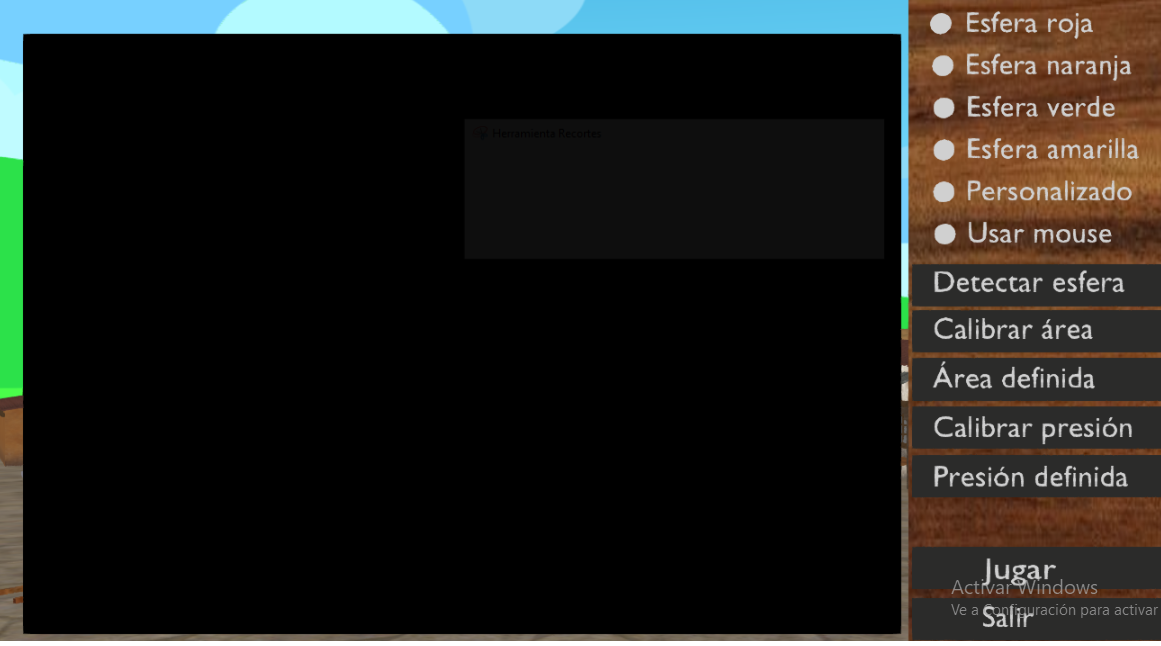
\includegraphics[scale=.35]{config_screen.PNG}
    \caption{Configuration Screen}
    \label{ConfScreen}
\end{figure}

Cada uno de los parámetros que se requiere en la pantalla de configuración cambia en el área donde está representado en la pantalla de configuracion, todos los juegos tienen una función al inicio que verifica si el mouse es el controlador principal o el tracker, lo mismo ocurre con el color del rastreador en la función del mismo.
\\
La aplicación web se ejecuta en un JSNode que ejecuta el nodo principal para conectar cada juego al Menú principal que se llama "Hacienda", toda la interfaz de la hacienda corre alrededor de una granja regional mexicana conocida como "hacienda", cada juego representa una tarea diferente en la hacienda, el primer juego que se implementó fue "Parrilla" donde el jugador realiza una serie de movimientos para simular la terapia que necesita. \\
\\
Toda la interfaz de "Hacienda" fue construida en blender, usando las utilidades Blend4Web, el menú principal fue diseñado completamente en Blender cada uno de los juegos esta representado en un objeto en el menú principal y en cada uno de ellos el modelo esta usando un layout de nodos vincula todos los juegos a la granja, cada juego tiene un Callback de JavaScript individual que se llama cuando el modelo vinculado se selecciona en la interfaz principal.
\begin{figure}[h]
    \centering
    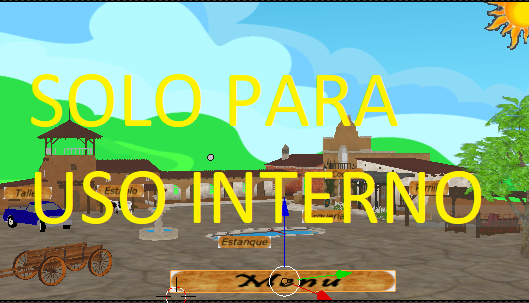
\includegraphics[scale=.7]{hacienda.PNG}
    \caption{"Hacienda"}
    \label{Hacienda}
\end{figure}
\\
En la versión Local de Gesture Therapy todos los juegos estaban programados en Blender usando el módulo de nodo, cuando se inició la propuesta de mover la versión local a una versión web, los problemas de compatibilidad comenzaron a mostrar la poca versatilidad del módulo, con el fin de minimizar la errores los módulos se borraron de casi todo el proyecto, y solo se dejaron en la interfaz principal y con el cambio de ser nodos Callback de llamada JS que usa la interfaz lógica ahora actual de los juegos, escribiendo los juegos usando la lógica anterior de los juegos  una tarea compleja que requiere imaginación y la capacidad de crear funciones para emular animaciones para los juegos sin olvidar preocuparse por la flexibilidad de los juegos y el movimiento de los usuarios.
\\
El primer juego en portar a la versión web fue "Parrilla", Parrilla es considerado por el staff del proyecto el mejor juego para introducir a nuevos usuarios a Gesture Therapy, la propuesta del juego es simple: el usuario simula estar asando hamburguesas y necesita voltear las hamburguesas deslizando la espátula debajo de la hamburguesa.
\\
El primer paso en el script es requerir todos los módulos del nodeJS que se van a utilizar.
\\
\begin{figure}[h]
    \centering
    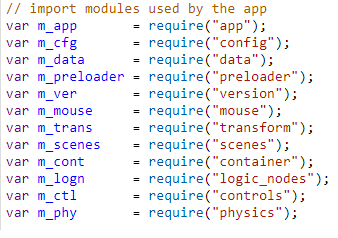
\includegraphics[scale=1]{modules.png}
    \caption{Modules}
    \label{Modules}
\end{figure}
Una de las desventajas de eliminar los nodos del juego es que el mouse ya no funciona, para poder programar todos los juegos en el script JS el siguiente paso fue hacer una estrategia de desarrollador de depurar el juego al mismo tiempo que se hace el script, la primera función que necesita atención es un detector de eventos para usar el movimiento del mouse en el juego, después de depurar y sincronizar el mouse con la espátula, luego debemos continuar con la lógica del juego.
\\
\begin{figure}[h]
    \centering
    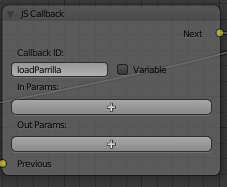
\includegraphics[scale=1.5]{parrilla_callback.PNG}
    \caption{CallBack}
    \label{CallBackParrilla}
\end{figure}
Utilizando Blender para modificar las características de los modelos, podemos seleccionar la hamburguesa junto a la espátula y crear a partir de cada uno de ellos un límite, en el caso de la hamburguesa seleccionamos un modelo en forma de  píldora para hacer que el límite del objeto sea un cilindro con bordes fileteados para facilitar el contacto con la espátula, en el caso de la espátula el límite elegido es una esfera en el centro de la parte plana del modelo, con esta configuración de los modelos la siguiente parte es configurar la colisión y el evento que va a suceder después de la colisión. \\

La acción tras la colisión sería una traslación de la hamburguesa a una coordenada aleatoria en la parrilla y una rotación a la mitad que se cocina para emular una animación de flip, tras la animación y la traslación procedemos a incrementar la puntuación.
\\
Con el juego casi terminado necesitamos implementar un temporizador para asegurarnos que el juego solo dure 60 segundos y mostrar ese valor en la pantalla en cualquier momento, junto al temporizador mostraríamos la puntuación en tiempo real.
\\
\begin{figure}[h]
    \centering
    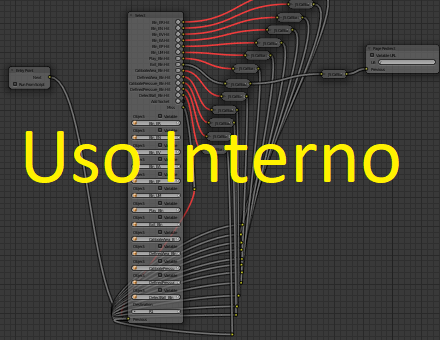
\includegraphics[scale=1.25]{Nodos.PNG}
    \caption{Nodes}
    \label{nodos}
\end{figure}
\section{Games}
\subsection{Parrilla}
\begin{figure}[h]
    \centering
    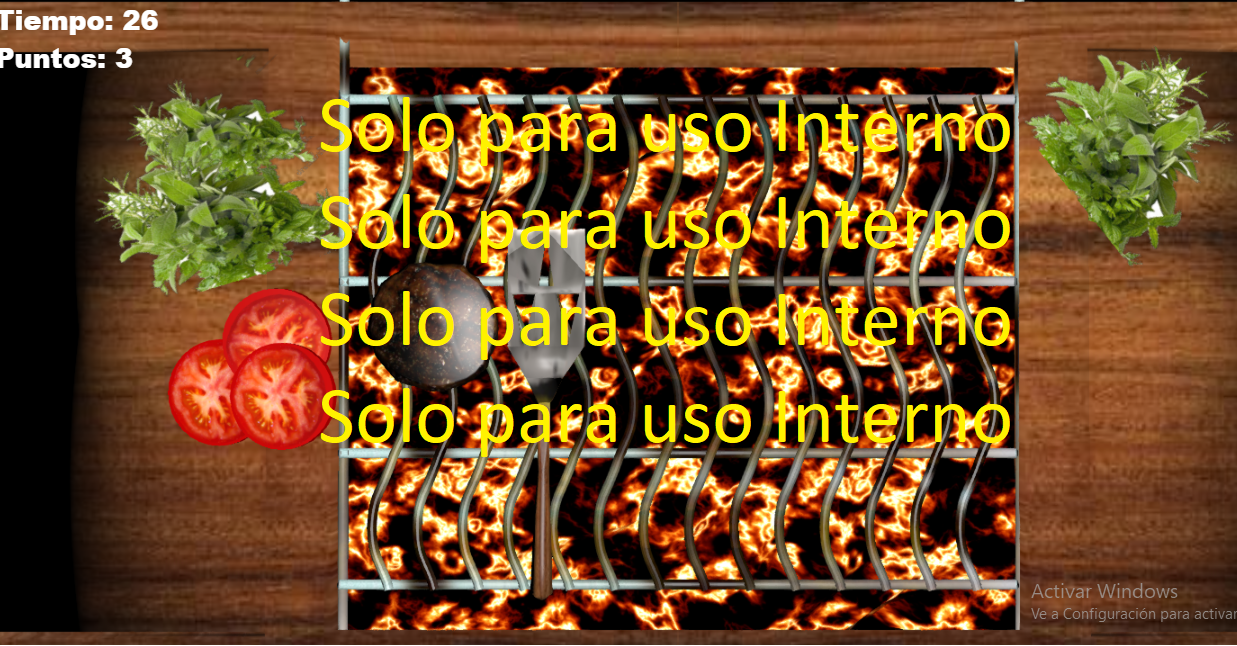
\includegraphics[scale=0.25]{parrilla.png}
    \caption{Parrilla Game }
    \label{parrilla}
\end{figure}
Antes de implementar el juego en JSNode, debemos asegurarnos de que el juego esté funcionando completamente y asegurarnos de que la interfaz principal esté conectada correctamente al juego que estamos probando, el archivo .blend debe configurarse con el callback de llamada adecuado para ejecutar el juego cuando se interactúa con el modelo. \\
\\
El segundo juego que se debió portear es Establo, este juego escala en nivel de complejidad con Parrilla, el objetivo en Establo es ordeñar una vaca para aumentar tu puntaje, como en el juego anterior los nodos fueron removidos y el scripting tiene hacerse desde cero, la ventaja de ser el segundo juego es que la mayoría de las funciones que creamos para Parrilla se pueden usar en Establo.
\\

Primero requerimos todos los módulos que se necesitan para importar las texturas y los modelos al juego, luego comenzamos a probar y reescribir los valores en nuestra función para controlar el avatar con el mouse, las funciones se mantienen iguales pero los parámetros de relación en pantalla y en el modelo son diferentes por lo que deben ajustarse,
\\
Una de las diferencias de este juego y el anterior es que este juego está en sistemas de coordenadas Z e Y, en este caso solo usaremos el eje Z para mover el avatar.
\\
\begin{figure}[h]
    \centering
    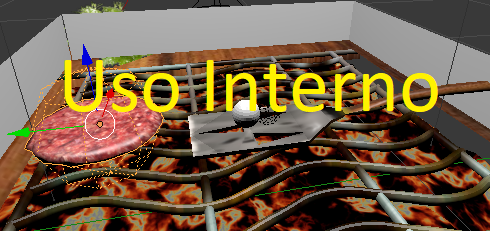
\includegraphics[scale=1]{bound_parrilla.png}
    \caption{Bound of the models in Parrilla}
    \label{Bounds}
\end{figure}
La naturaleza del juego es ordeñar a la vaca, para lograr el objetivo en esta tarea el usuario necesita agarrar la ubre de la parte superior y arrastrarla hacia la parte inferior para ordeñar con éxito a la vaca, el primer objetivo a programar es una bandera condicional que se habilita cuando se agarra la parte superior de la ubre, para asegurar que el usuario está presionando el sensor de del gripper, para evaluar esta condición se verifican las coordenadas en el eje Z del avatar y se registra en mi momento que el usuario comienza a agarrar, guardando el valor de la Z al principio y registrándolo nuevamente cuando la suelta, la animación y la puntuación aumentan solo si los valores iniciales de Z están por encima de un parámetro arbitrario fijo y el valor de Z final está por debajo de otro fijo parámetro arbitrario. \\
Debido a la naturaleza de la tarea en el juego, todos los objetos se colocaron  para lograr la perspectiva del usuario y ninguno de los modelos choca realmente.
\begin{figure}[h]
    \centering
    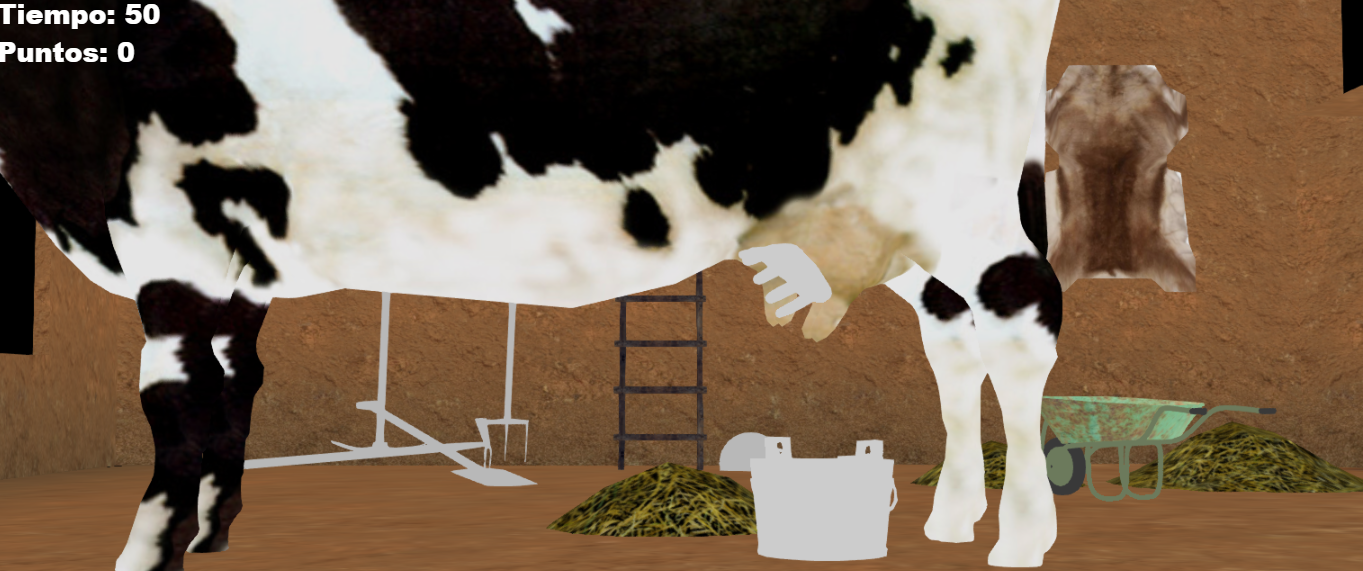
\includegraphics[scale=0.35]{establo.png}
    \caption{Establo}
    \label{Establo}
\end{figure}
\end{document}
